\section{Conexión entre la Raspberry Pi y el Router}


Para que la Raspberry Pi pueda tener comunicación con el Router, se procedió a colocar una ip fija en la Raspberry Pi, para ello se utilizó el siguiente comando:
\begin{lstlisting}[style=terminal]
sudo nano /etc/netplan/50-cloud-init.yaml

\end{lstlisting}

Contenido del archivo 50-cloud-init.yaml:

\begin{lstlisting}[style=terminal]
network:
  version: 2
  ethernets:
    eth0:
      dhcp4: no
      dhcp6: no
      addresses:
        - 192.168.10.1/24

\end{lstlisting}

Luego de esto, se procedió de igual manera configurando una ip en el puerto del router que se encuentra conectado a la Raspberry Pi, para ello se utilizó el siguiente comando:
\begin{lstlisting}[style=terminal]
<Huawei>system-view
[Huawei]interface GigabitEthernet 0/0/0
[Huawei-GigabitEthernet0/0/0]undo portswitch
[Huawei-GigabitEthernet0/0/0]ip address 192.168.10.2 255.255.255.0
[Huawei-GigabitEthernet0/0/0]quit

\end{lstlisting}



\section{Configuración de SNMP en el Router}
\begin{itemize}
  \item Se activa SNMP

\begin{lstlisting}[style=terminal]
<Huawei>system-view
[Huawei]sysname Router-Monitoreado
[Router-Monitoreado]snmp-agent permit interface GigabitEthernet0/0/0
[Router-Monitoreado]snmp-agent
[Router-Monitoreado]snmp-agent sys-info version v3

\end{lstlisting}

Para monitorear interfaces, tráfico, información del sistema y otros recursos, se crea una vista.
\begin{lstlisting}[style=terminal]
[Router-Monitoreado]snmp-agent mib-view netdata-view include iso

\end{lstlisting}


El parámetro \texttt{include} indica que el subárbol especificado será
incorporado dentro de la vista permitida, mientras que \texttt{iso} representa
el nodo raíz del árbol de identificadores de objetos SNMP, equivalente al OID
\texttt{1}. Por lo tanto, esta configuración permite que Netdata consulte tanto
las MIB estándar, utilizadas para obtener información del sistema, interfaces,
tráfico, errores y tiempo de actividad, como las MIB empresariales propias de
Huawei.




\item Crear el grupo SNMPv3



\begin{lstlisting}[style=terminal]
[Router-Monitoreado]snmp-agent group v3 netdata-group privacy read-view netdata-view
\end{lstlisting}

- v3: utiliza SNMPv3.\\
- privacy: exige autenticación y cifrado.\\
- read-view netdata-view: concede acceso de lectura a la vista creada. \\
- No se configura write-view, porque Netdata solamente necesita consultar información. \\


\item Crear el usuario SNMPv3 y asignarlo al grupo creado anteriormente.


\begin{lstlisting}[style=terminal]
[Router-Monitoreado]snmp-agent usm-user v3 netdata-user group netdata-group
\end{lstlisting}


\begin{lstlisting}[style=terminal]
[Router-Monitoreado]snmp-agent usm-user v3 netdata-user authentication-mode sha2-256
\end{lstlisting}
El router pedira contraseña para el usuario, se ingresa la contraseña deseada y se confirma. En este caso se utilizó la contraseña \texttt{NetAuth2026}.

\begin{lstlisting}[style=terminal]
[Router-Monitoreado1]snmp-agent usm-user v3 netdata-user privacy-mode aes128
\end{lstlisting}

El router pedira contraseña para el usuario, se ingresa la contraseña deseada y se confirma. En este caso se utilizó la contraseña \texttt{NetPriv2026}.

\item Comprobar la configuración de SNMPv3 con el siguiente comando:
\begin{lstlisting}[style=terminal]
[Router-Monitoreado]display snmp-agent usm-user

[Router-Monitoreado]quit
<Router-Monitoreado>save
\end{lstlisting}

\begin{figure}[H]
    \centering
    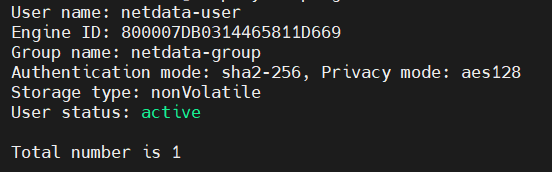
\includegraphics[scale= 0.9]{Pictures/SNM1.png}
    \caption{Confirmación de configuración de SNMPv3 en el Router}
    
\end{figure}



\item Para comprobar que la Raspberry Pi puede comunicarse con el Router, se utilizó el siguiente comando:

Primero se deben de instalar los paquetes necesarios para poder utilizar el comando \texttt{snmpwalk}:
\begin{lstlisting}[style=terminal]
sudo apt update
sudo apt upgrade
sudo apt install -y snmp
\end{lstlisting}

\begin{lstlisting}[style=terminal]
snmpwalk -v3 \
  -l authPriv \
  -u netdata-user \
  -a SHA-256 \
  -A 'NetAuth2026'' \
  -x AES \
  -X 'NetPriv2026' \
  192.168.10.2 \
  1.3.6.1.2.1.1
\end{lstlisting}


\begin{figure}[H]
    \centering
    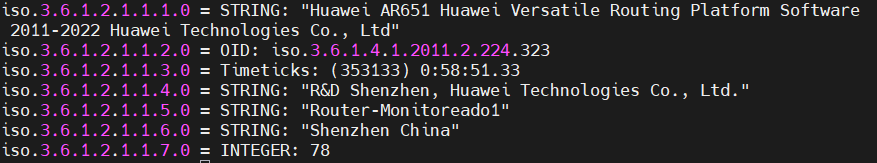
\includegraphics[scale= 0.9]{Pictures/SNM12.png}
    \caption{Confirmación de lectura de información del Router desde la Raspberry Pi}

\end{figure}

\end{itemize}



\section{Configuración de Netdata para recibir al router}


\begin{itemize}

  \item El archivo de configuración de SNMP se encuentra en la siguiente ruta: \\
  \texttt{/etc/netdata/go.d/snmp.conf}. Para editarlo se utiliza el siguiente comando:
\begin{lstlisting}[style=terminal]
sudo nano /etc/netdata/go.d/snmp.conf
\end{lstlisting}



  \item Se utiliza el siguiente contenido para el archivo de configuración de SNMP:
\begin{lstlisting}[style=terminal]

jobs:
  - name: huawei_router
    hostname: 192.168.10.2
    update_every: 60
    timeout: 5

    options:
      version: 3

    user:
      name: netdata-user
      level: authPriv
      auth_proto: sha256
      auth_key: "NetAuth2026"
      priv_proto: aes
      priv_key: "NetPriv2026"


\end{lstlisting}

Si se desea monitorear más de un router, se puede agregar otro bloque de configuración con el mismo formato, cambiando el nombre del trabajo y la dirección IP del router correspondiente.


  \item Luego de cerrar el archivo, se colocó seguridad de que el archivo de configuración de SNMP tenga los permisos correctos, para ello se utilizó el siguiente comando:


\begin{lstlisting}[style=terminal]
sudo chown root:netdata /etc/netdata/go.d/snmp.conf
sudo chmod 640 /etc/netdata/go.d/snmp.conf
\end{lstlisting}


  \item Luego de estos pasos, se debe de reiniciar el servicio de Netdata para que los cambios surtan efecto, para ello se utilizó el siguiente comando:
\begin{lstlisting}[style=terminal]
  sudo systemctl restart netdata
  \end{lstlisting}

  
 \item Al ingresar a la interfaz web de Netdata, se puede observar que el router se encuentra monitoreado y se puede visualizar información como tráfico, errores, tiempo de actividad, entre otros.

\begin{figure}[H]
    \centering
    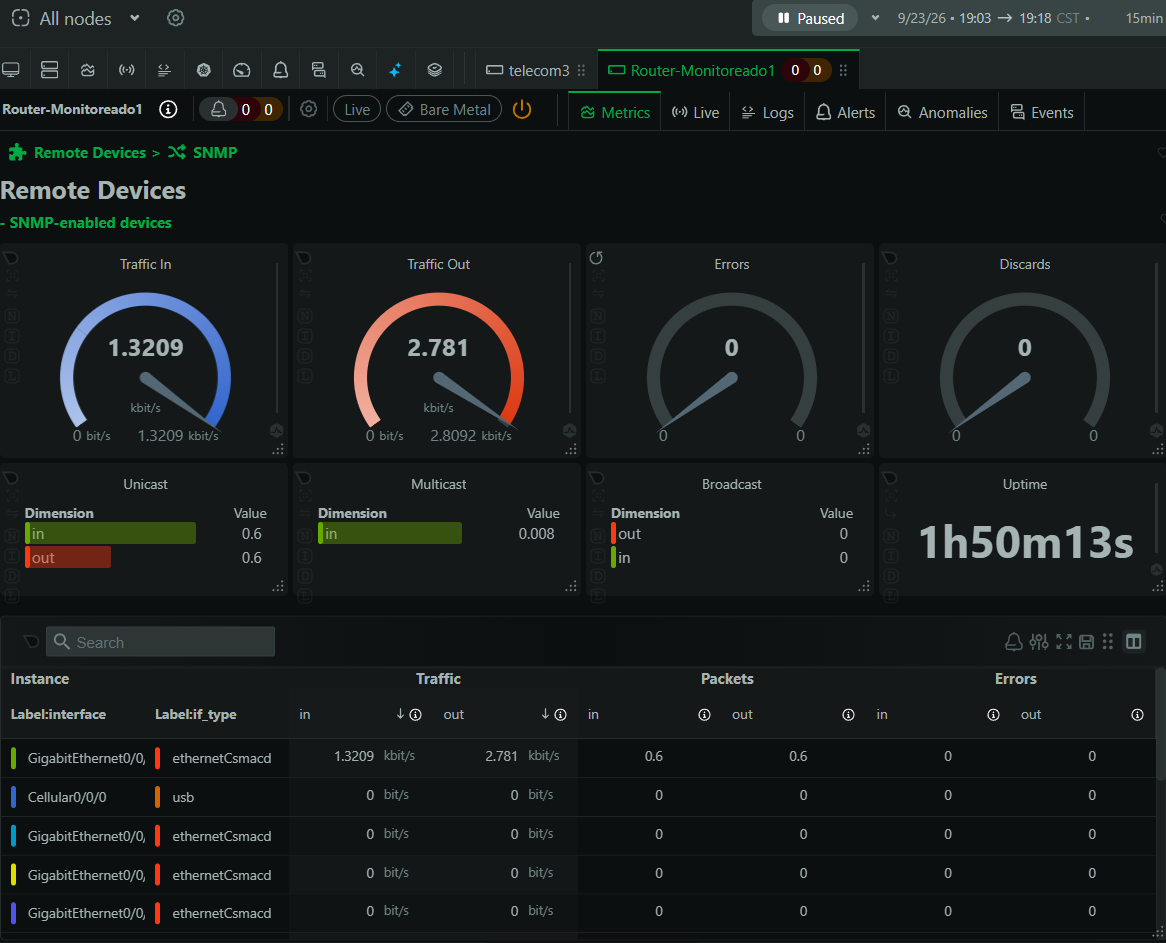
\includegraphics[scale= 0.6]{Pictures/SNM3.png}
    \caption{Interfaz web de Netdata mostrando información del router monitoreado}
  
\end{figure}

\end{itemize}


Estos mismos pasos se realizan para todos los demás routers que se deseen monitorear, cambiando únicamente la dirección IP del router y el nombre del router y el nombre del trabajo en el archivo de configuración de SNMP. (El nombre que muestra Netdata es el nombre del router que se configuró en el router, en este caso \texttt{Router-Monitoreado}).